\documentclass[conference]{IEEEtran}
\IEEEoverridecommandlockouts
% The preceding line is only needed to identify funding in the first footnote. If that is unneeded, please comment it out.
\usepackage{cite}
\usepackage{amsmath,amssymb,amsfonts}
\usepackage{algorithmic}
\usepackage{graphicx}
\usepackage{textcomp}
\usepackage{xcolor}

\usepackage{setspace}
\usepackage[T1]{fontenc}
\usepackage{url}
\usepackage{hyperref}
\usepackage{enumitem}
\usepackage{mathtools}
\def\BibTeX{{\rm B\kern-.05em{\sc i\kern-.025em b}\kern-.08em
		T\kern-.1667em\lower.7ex\hbox{E}\kern-.125emX}
}
\newcounter{boxlblcounter}  
\newcommand{\makeboxlabel}[1]{{#1.}\hfill}% \hfill fills the label box
\newenvironment{boxlabel}
{\begin{list}
		{\arabic{boxlblcounter}}
		{\usecounter{boxlblcounter}
%			\setlength{\labelwidth}{3em}
%			\setlength{\labelsep}{0em}
			\setlength{\itemsep}{2pt}
			\setlength{\leftmargin}{1cm}
%%			\setlength{\rightmargin}{2cm}
%			\setlength{\itemindent}{0em} 
			\let\makelabel=\makeboxlabel
		}
	}
{\end{list}}
\usepackage{caption}

\usepackage{fourier}
\usepackage{bookmark}
\usepackage{array}
\usepackage{listings}
\usepackage{float}
\usepackage{pifont}% http://ctan.org/pkg/pifont
\newcommand{\xmark}{\ding{55}}%

\begin{document}
	
	%%
	%% Modified title page for UA
	\begin{titlepage}
	\begin{figure}[t]
		\begin{minipage}{\textwidth}
			\centering
			
\includegraphics[scale=0.35]{Images/UA/OfficLogo-Engineering.png}
		\end{minipage}
	\end{figure}

	\quad\\
	\vspace{0.5in}
	\centering
	\begin{spacing}{2.0}
		{ \textbf{\LARGE AVoIP: Ad-Hoc Voice over Internet Protocol for Small Single-board Computers}}
	\end{spacing}
	
	\vspace{1.5in}
	\textbf{\Large Term Project Proposal}
	\vspace{3.0in}

	\begin{minipage}{0.49\textwidth}
		\begin{flushleft}
			\textit{{Students:}} \\
			{\textbf{Trupeshkumar R. Patel}}\\
			\textsl{trpatel2@crimson.ua.edu}\\
			{\textbf{David Coleman}}\\
			\textsl{dmcoleman1@crimson.ua.edu}\\
			{\textbf{Xiaoming Guo}}\\
			\textsl{xguo29@crimson.ua.edu}
		\end{flushleft}
	\end{minipage}
	\begin{minipage}{0.5\textwidth}
		\begin{flushright}
			\textit{{Supervisor:}} \\
			{\textbf{Dr. Xiaoyan Hong}}\\
			\textsl{hxy@cs.ua.edu}
		\end{flushright}
	\end{minipage}

	\begin{figure}[b]
		\begin{minipage}{0.55\textwidth}
			\begin{flushleft}
				\textbf{\large Department of Computer Science}
			\end{flushleft}
		\end{minipage}
		\hfill
		\begin{minipage}{0.35\textwidth}
			\begin{flushright}
				\textsc{\textbf{\today}}
			\end{flushright}
		\end{minipage}
	\end{figure}

\end{titlepage}
	
	%%
	%% The "title" command has an optional parameter,
	%% allowing the author to define a "short title" to be used in page headers.
	\title{VoIP: Voice over Internet Protocol for Small Single-board Computers}
	\IEEEspecialpapernotice{(Final Report)}
	%%
	%% The "author" command and its associated commands are used to define
	%% the authors and their affiliations.
	%% Of note is the shared affiliation of the first two authors, and the
	%% "authornote" and "authornotemark" commands
	%% used to denote shared contribution to the research.
	%\author{
%	\IEEEauthorblockN{Trupesh R. Patel}
%	\IEEEauthorblockA{
%		Department of Computer Science\\
%		College of Engineering\\
%		\textit{University of Alabama}\\
%		Tuscaloosa, AL 35487\\
%		trpatel2@crimson.ua.edu\\
%%		\orcid{0000-0003-4321-6699}
%	}
%
%	\and
%	
%	\IEEEauthorblockN{Author 1}
%	\IEEEauthorblockA{
%		Department
%		\textit{University of Alabama}\\
%		Tuscaloosa, AL 35487\\
%		email@email.com
%%		\orcid{0000-0003-4321-6699}
%	}
%
%	\and
%	
%	\IEEEauthorblockN{Author 2}
%	\IEEEauthorblockA{
%		Department
%		\textit{University of Alabama}\\
%		Tuscaloosa, AL 35487\\
%		email@email.com
%		%		\orcid{0000-0003-4321-6699}
%	}
%}



\author{
	\IEEEauthorblockN{
		Trupesh R. Patel\IEEEauthorrefmark{1}, 
		David Coleman\IEEEauthorrefmark{1}, 
		Xiaoming Guo\IEEEauthorrefmark{1}
	} 
	\IEEEauthorblockA{
		\IEEEauthorrefmark{1}Department of Computer Science\\
					College of Engineering\\
					\textit{University of Alabama}\\
					Tuscaloosa, AL 35487\\
					$\left\{trpatel2,\ dmcoleman1,\ xguo29\right\}$@crimson.ua.edu
	} 
}


	
	%%
	%% This command processes the author and affiliation and title
	%% information and builds the first part of the formatted document.
	\maketitle
	\thispagestyle{plain}
	\pagestyle{plain}
	
	%%
	%% The Abstact is a short summary of the work to be presented in the
	%% article.
	\begin{abstract}
	\label{sec:abstract}
		Asterisk PBX~\cite{sangoma-technologies} is an implementation of IP-PBX software, a digital version of Private Branch Exchange (PBX) technology, meant for IP networks instead of traditional telephone networks. IP-PBX software allows for the setup of VoIP (Voice over Internet Protocol) communications on computers and mobile devices, and can be run on less powerful devices such as Raspberry Pi. However, using smaller single-board devices come with the limitation of computing power and storage capacity. As a result of these limitations, packets can be dropped at a great rate, cutting off VoIP callers when a Pi needs to handle a significant number of calls simultaneously. In this project, the authors provides test the Raspberry Pi's suitability for providing IP-PBX services by analyzing the packets delays, network jitters, end-to-end network latency, and bandwidth between an Asterisk PBX system installed on Raspberry Pi 4~\cite{cytron-technologies} and IP clients that are using VoIP as service. This analysis is performed by testing the system with clients at varying distances from the Raspberry Pi.
\end{abstract}
	
	%%
	%% Keywords. The author(s) should pick words that accurately describe
	%% the work being presented. Separate the keywords with commas.
%	\begin{IEEEkeywords}
%		abc
%	\end{IEEEkeywords}
	
	%%
	%% The introdution section
	\section{Introduction \& Background}	
\label{sec:introduction-background}
Voices can have multiple functions among the information flowing at the edge of the IoT network. They can carry valuable content, reflect the conditions of an environment, and can be used to command other entities through acoustic actuators and phone calls. However, implementing voice systems at the edge of such networks typically faces challenges, namely that edge devices are always constrained by computing power, bandwidth contention, and energy consumption. Therefore, it is not feasible to implement a complete TCP/IP stack on each node and give all nodes the ability to connect to remote entities outside the local network.

IP-PBX (IP-based Private Branch Exchange) provides a comprehensive solution to address the aforementioned issues. As the analog equivalent of IP PBX, the design of the traditional PBX system is to serve a private organization, in which both the geographic area and the communication connection are limited to a specific scope. Connections between internal phones are without cost, while only central office lines provide connections to the public switched telephone network (PSTN). This scheme meets our expectations for edge IoT communication -- internal communication does not occupy egress bandwidth, and some switcher servers still reserve the communication egress to the outside. Leveraging VoIP technology, IP-PBX has ported the PBX scheme to the Internet, replacing telephone lines with packet-switching networks. The IP-based paradigm offers better scalability and lowers the cost same as the Internet brings to other domains. 

Several mature implementations of the IP-PBX paradigm are available, including 3CX~\cite{3cx_2022} and Asterisk PBX~\cite{sangoma-technologies}. Asterisk is an open-source software package that can run all PBX functions, along with some other functions, usually on a Linux operating system platform. Voicemail services, conference calling, interactive voice response, and call queuing are provided by Asterisk, along with the essential telephony services. It also provides multi-party calling and displaying of caller ID (display calling number). To interact with digital telephone equipment and analog telephone equipment, Asterisk needs the support of PCI hardware, the most famous of which is provided by the Digium platform. 

From the architecture perspective, Asterisk serves as a middleware function, connecting the underlying telephony technology and the upper-level telephony applications. Both PBX and IVR (Interactive Voice Response) functionalities are integrated within Asterisk. Using compatible PCI hardware, Asterisk supports traditional telephone lines, including TDM (Time Division Multiplexing), TI/El PRI/PRA\&RBS (Robbed Bit Signal) mode, analog telephone line/analog telephone (POTS), ISDN (Integrated Services Digital Network) and BRI (Basic Rate) and PRI (Primary Rate). Also, due to the PCI hardware support feature, Raspberry Pi can be used to implement the Asterisk instance. 

By using small single-board computers such as Raspberry Pi, any types of businesses can deploy the cost affordable IP based PBX system. Raspberry Pi is small and light weight device, and runs on low power consumption. Having it for single tasks like allowing for VoIP by running Asterisk PBX is a very easy and economical. However, because this device is smaller and lighter, it can only handle a limited number of tasks. This paper will analyze the boundaries of the Raspberry Pi by packets delays, network jitters, end-to-end network latency, and bandwidth of calls made at varying distances from the Pi to determine how effectively IP-PBX services can be run on such devices.
	
This paper is organized into specific sections. \hyperref[sec:setup]{Section \ref{sec:setup}} lists the required hardware and software involved with the experiments performed here.  \hyperref[sec:obstacles]{Section \ref{sec:obstacles}} explains the obstacles faced when setting up for the tests in this experiment. \hyperref[sec:analysis-methods]{Section \ref{sec:analysis-methods}} explains the protocols that Asterisk PBX is using to connect devices and forward calls, how the calls are impacted by different network issues, and what topology IP-PBX services utilize to connect devices. \hyperref[sec:experiments]{Section \ref{sec:experiments}} shows detailed description for each experiment performed. \hyperref[sec:future-work]{Section \ref{sec:future-work}} goes over different ways the material of this paper can be expanded upon in the future. Finally, \hyperref[sec:conclusion]{Section \ref{sec:conclusion}} concludes the paper, giving an overview of the results seen thus far.
	
	%%
	%% The Software and Hardware Setup section
	\section{Software \& Hardware Setup}	\label{sec:setup}
	abc

	%%
	%% The Obstacles section
	\section{Obstacles} \label{sec:obstacles}
    \subsection{Local Network Issues}
        An initial problem found when working with PBX software was configuring connections for the device hosting it and for the devices that are connected with it (e.g. smart phones and computers). As IP-PBX uses IP networks for its functionality, a single local network was used for testing the functionality of the Raspberry Pi, which the Pi itself and all machines running VoIP software were connected to, Eduroam. Eduroam is the primary wireless network used within the University of Alabama campus, with access points in each building, allowing devices across buildings to stay on one local area network. 
        
        This provided a few benefits to the experiment, most prominently allowing for VoIP calls to be made from greater distances (i.e. from a different building) while simplifying the process of connecting devices to the Raspberry Pi. However, an issue found with this was that Eduroam was not initially allowing the Pis to connect. An additional script was required to sign into the network as students. After the script was ran and the Pis rebooted, they could freely join the network afterward.
        
        \begin{figure}[htbp]
			\centerline{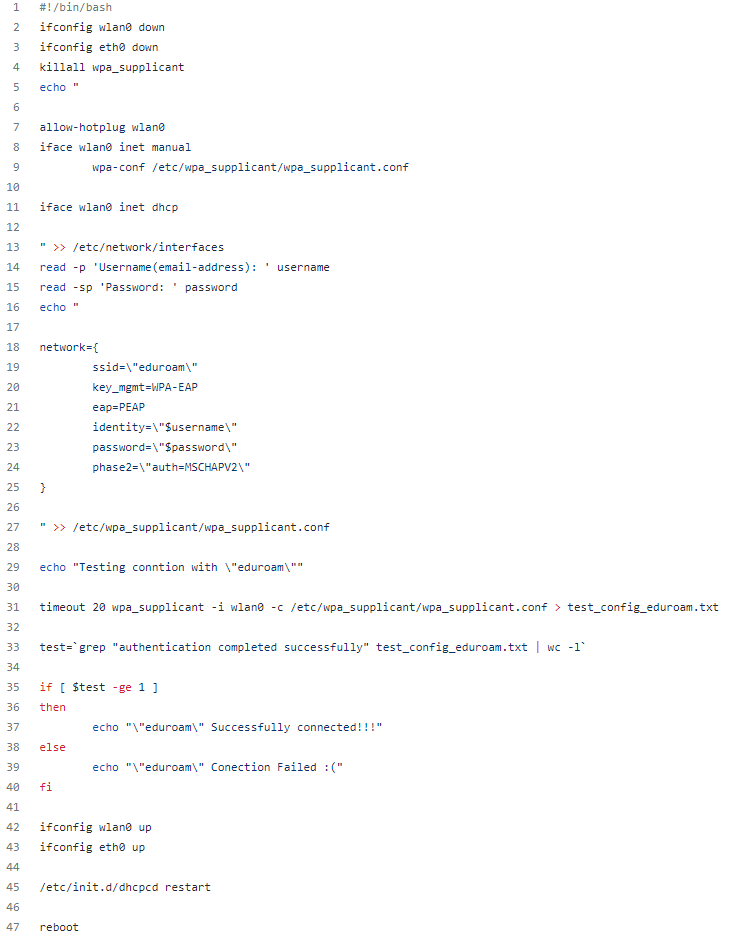
\includegraphics[width=8cm]{Images/experiment/eduroam.PNG}}
			\caption{Script used to join Eduroam network}
			\label{fig:edu-script}
		\end{figure}
		
		Another problem more central to the use of IP-PBX software is the complication of connecting remote devices to the Raspberry Pi. Within Eduroam, VoIP software only required the domain of the Raspberry Pi within the local area network to register on the IP-PBX software the Pi was running. However, if the device was on a different network, it proved incapable of finding the Pi as easily. There are a few possible explanations for this, such as there being a firewall blocking most traffic outside of Eduroam or NAT changing the IP of the Pi from outside Eduroam. Without the ability to make calls from different networks, making long distance VoIP calls proved to be quite limited, and the available tests for the Raspberry Pi were limited. While this issue may have been resolved with further research, it was ultimately decided that having all devices connect to Eduroam still allowed for enough trials to analyze the Pis functionality in running IP-PBX software.
		
	\subsection{Complexity of IP-PBX}
	    IP-PBX proved to be quite complex in setup and configuration. Asterisk PBX, a mature open-source implementation, was utilized. Initial compilation of Asterisk showed that there were many options on modules to be used, many of which were extraneous. After setup was done, the PBX needed to be further configured to allow for distinct users to be registered, to denote what should be done if a call was made to a certain number, and to dictate what kind of channel to use for SIP. Determining what configuration files needed to be used and changed and in what ways was a major obstacle in beginning the testing of the Raspberry Pi.
	    
	    \begin{figure}[htbp]
			\centerline{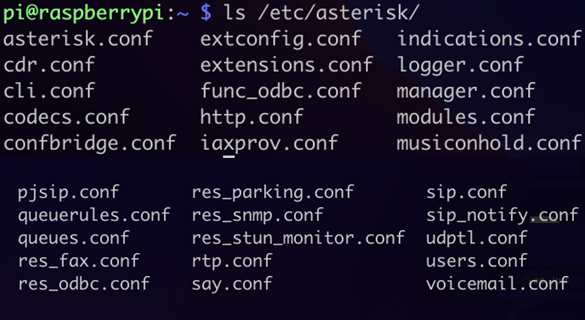
\includegraphics[width=8cm]{Images/experiment/config.png}}
			\caption{The configuration files for Asterisk PBX. Note that the majority of edits needed to be made to sip.conf and extensions.conf}
			\label{fig:conf}
		\end{figure}
		
	\subsection{Abundance of Third Party Software}
	    Many pieces of third party software needed to be utilized to conduct these tests, each adding more setup time and complication to the experiments. Asterisk PBX needed to be downloaded onto the Raspberry Pi to allow the Pi to provide IP-PBX services. Zoiper was needed to make VoIP calls and register devices on the Pi for IP-PBX services, with MicroSIP and Telephone needed to make additional calls, as Zoiper limits the number of free users. Wireshark was required to gather more information on the packets sent to and from the Pi while hosting calls to analyze its performance. Additionally, other services, such as SIP.US (used for SIP trunking) and Clumsy (used for network emulation) were considered for use until they were deemed unnecessary. The number of extraneous services utilized exacerbated the complexity of performing these experiments. enefits to the experiment, most prominently allowing for VoIP calls to be made from greater distances (i.e. from a different building) while simplifying the process of connecting devices to the Raspberry Pi. However, an issue found with this was that Eduroam was not initially allowing the Pis to connect. An additional script was required to sign into the network as students. After the script was ran and the Pis rebooted, they could freely join the network afterward.
	
	%%
	%% The Analysis Method section
	\section{Analysis \& Methods}	\label{sec:analysis-methods}
Due to the inherent characteristics of the VOIP (Voice over IP) application, a series of protocols and mechanisms have been designed to ensure the quality of VoIP communication. One task of the experiments is protocol research, including analyzing the collaboration between the protocols included in the process and finding out the principles of the VoIP application design.

According to the "branch exchange" scheme, the first step is building the link, of which the responsibility is taken by the Session Initiation Protocol (SIP).


\subsection{Basic SIP Analysis}
The Session Initiation Protocol (SIP) is an application layer control protocol for establishing, changing and terminating multimedia sessions, where the sessions can be IP telephony, multimedia sessions or multimedia conferences. SIP is the core protocol of many IP-based PBX applications, including Asterisk.

\begin{figure}[htbp]
	\centerline{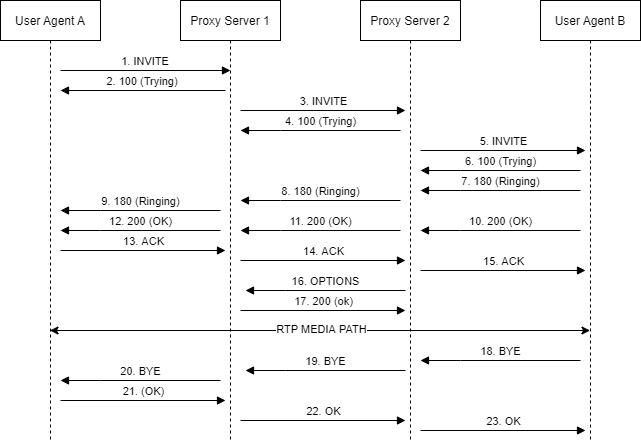
\includegraphics[width=8cm]{Images/experiment/SIP.png}}
	\caption{Session Initialization in SIP model}
	\label{fig:sip}
\end{figure}



As shown in Fig.\ref{fig:sip}, the SIP process starts with registration. All SIP terminals as User Agents should register with the registration server to inform their location, session capability, and other information.

Usually, when the SIP terminal (User Agent) is powered on or configured to perform a registration operation, a registration request message (REGISTER) is sent to the registration server, carrying all the information that needs to be registered. After receiving the registration request message, the registration server sends a response message to the terminal to inform it that the request message has been received. If the registration is successful, it will send a "200 OK" message to the terminal. However, the most common response is a "401 Unauthorized" message because authorization is required in most of the implementations for security purposes. 

The SIP protocol adopts the Client-Server pattern, in which the calls are established between User Agents through the proxy server.

Upon the link built by SIP, the data transmission tasks are carried out with RTP/RTCP protocol.

\subsection{RTP}
RTP is a real-time protocol for transmitting audio and video streams over IP networks. For telephony applications, the data consists of voice spurts, instead of being a stable data flow. So each RTP packet only contains a small sample of voice messages, whose length is usually 20 to 30 ms.

RTP introduces two fields into its header, the sequence number and the timestamp, generated by the sender devices.

\subsection{RTCP}
RTCP is a control protocol accompanied by RTP, providing the report of the RTP stream received by the destination devices. So RTCP packets always head in the reverse direction of RTP streams. After checking the RTCP report, the sender updates the transmission strategy to adapt to the network condition.

\subsection{Jitter and Packet loss}
VoIP applications are sensitive to jitter. In VoIP calls, the voice stream consists of alternating talk spurts and silent periods. Since silent periods separate the discrete valuable voice messages, the timing and the sequence of the packets' arrival are very important. Voice packets that are out of order may not be decoded correctly. Jitter has a large impact on the sequence of the arriving RTP packets. If the packets arrive at even intervals in the correct order, the jitter is low. Reversely, if the packets arrive in bursts or out of order, the jitter is high.

Compared with jitter, packet loss can be tolerant because it does not change the sequence and time of the packet. So the packet loss that is under a threshold, usually under 3\% can be accepted.

In the experiment, jitter has been applied as an important indicator to evaluate the quality of the VoIP calls.


\subsection{Basic Network Topology}
To demonstrate the main components of the SIP communication, a simplified scenario is implemented, as shown in Figure  \hyperref[fig:topo]{Figure \ref{fig:topo}}. Two VoIP applications are running on the same computer, and an IP-based PBX application (Asterisk), running on a Raspberry Pi 4, is serving as the PBX server.

\begin{figure}[htbp]
	\centerline{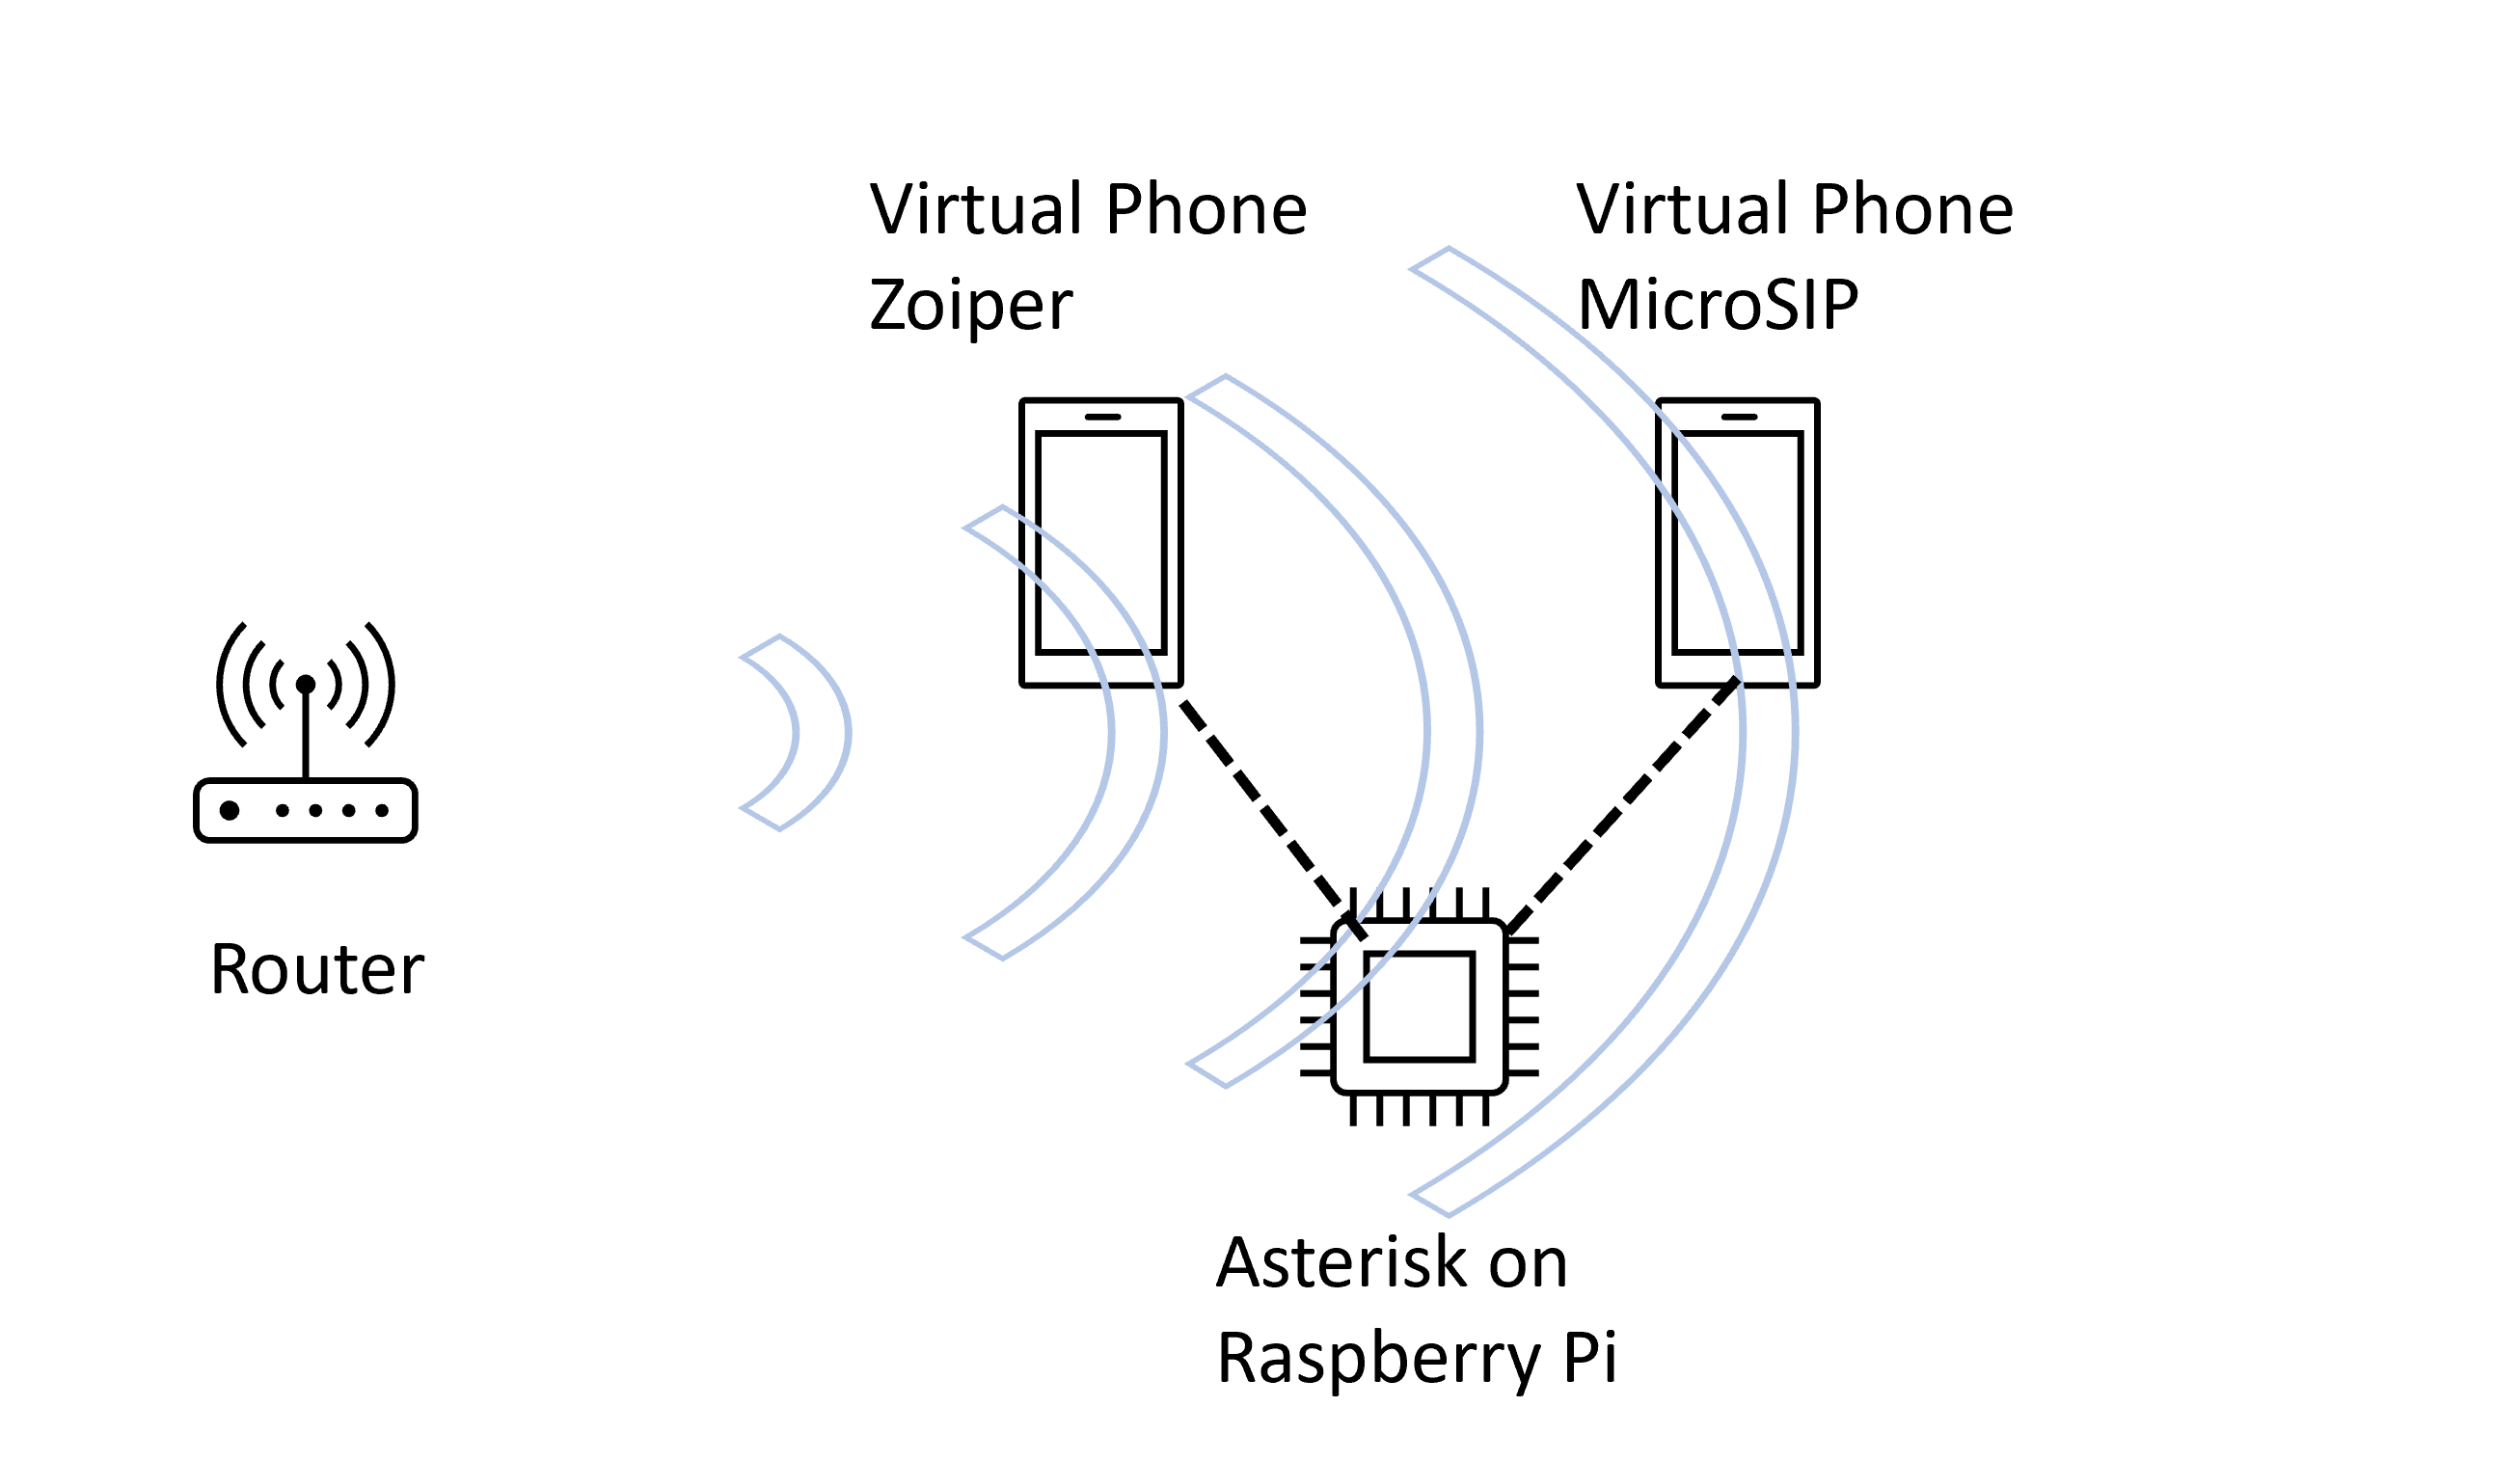
\includegraphics[width=8cm]{Images/experiment/exp1.png}}
	\caption{Simplified Scenario}
	\label{fig:topo}
\end{figure}

To trace and see all types of packets transmissions, author used Wireshark open-source software. \hyperref[fig:packet-trace]{Figure \ref{fig:packet-trace}} is a flow sequence of the one single call from Zoiper5 user (IP: 192.168.60.106:63771) to MicroSIP user (IP:192.168.60.106:53493). In this, scenario their are actual two connections, first from Zoiper5 user to Asterisk (shown in left-side of Figure \ref{fig:packet-trace}) and second Asterisk to MicroSIP (shown in right-side of Figure \ref{fig:packet-trace}).

\begin{figure}[htbp]
	\begin{minipage}{0.24\textwidth}
		\begin{flushleft}
			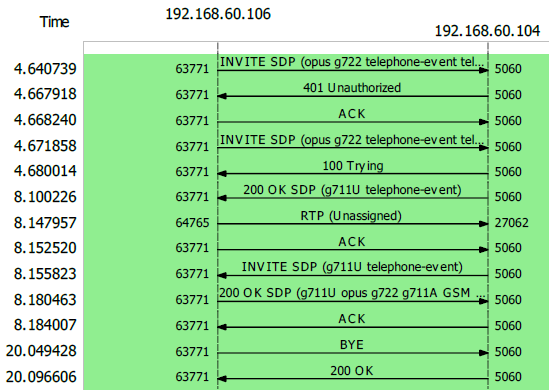
\includegraphics[height=100pt,width=\textwidth]{Images/experiment/a1.png}
			%%					\caption{Zoiper to Asterisk}
		\end{flushleft}
	\end{minipage}
	\begin{minipage}{0.24\textwidth}
		\begin{flushright}
			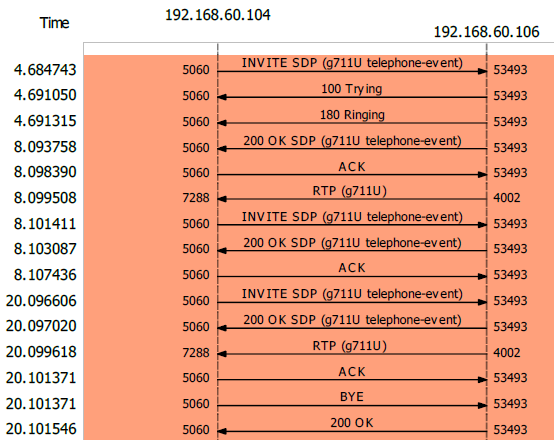
\includegraphics[height=100pt,width=\textwidth]{Images/experiment/a2.png}
			%					\caption{Zoiper to MicroSIP}
		\end{flushright}
	\end{minipage}
	\caption{SIP packet transmission from Zoiper to Asterisk(left-side), Asterisk to MicroSIP (right-side)}
	\label{fig:packet-trace}
\end{figure}
	
	%%
	%% The Experiment section
	\section{Experiment}	
\label{sec:sip}


\subsection{Basic SIP Analysis}

The Session Initiation Protocol (SIP) is an application layer control protocol for establishing, changing and terminating multimedia sessions, where the sessions can be IP telephony, multimedia sessions or multimedia conferences. SIP is the core protocol of many IP-based PBX applications, including Asterisk.

To demonstrate the main components of the SIP communication, a simplified scenario is implemented, as shown in Figure \ref{fig:topo}. Two softphone applications are running on the same computer, and an IP-based PBX application (Asterisk), running on a Raspberry Pi 4, is serving as the PBX server.

\begin{figure}[htbp]
\centerline{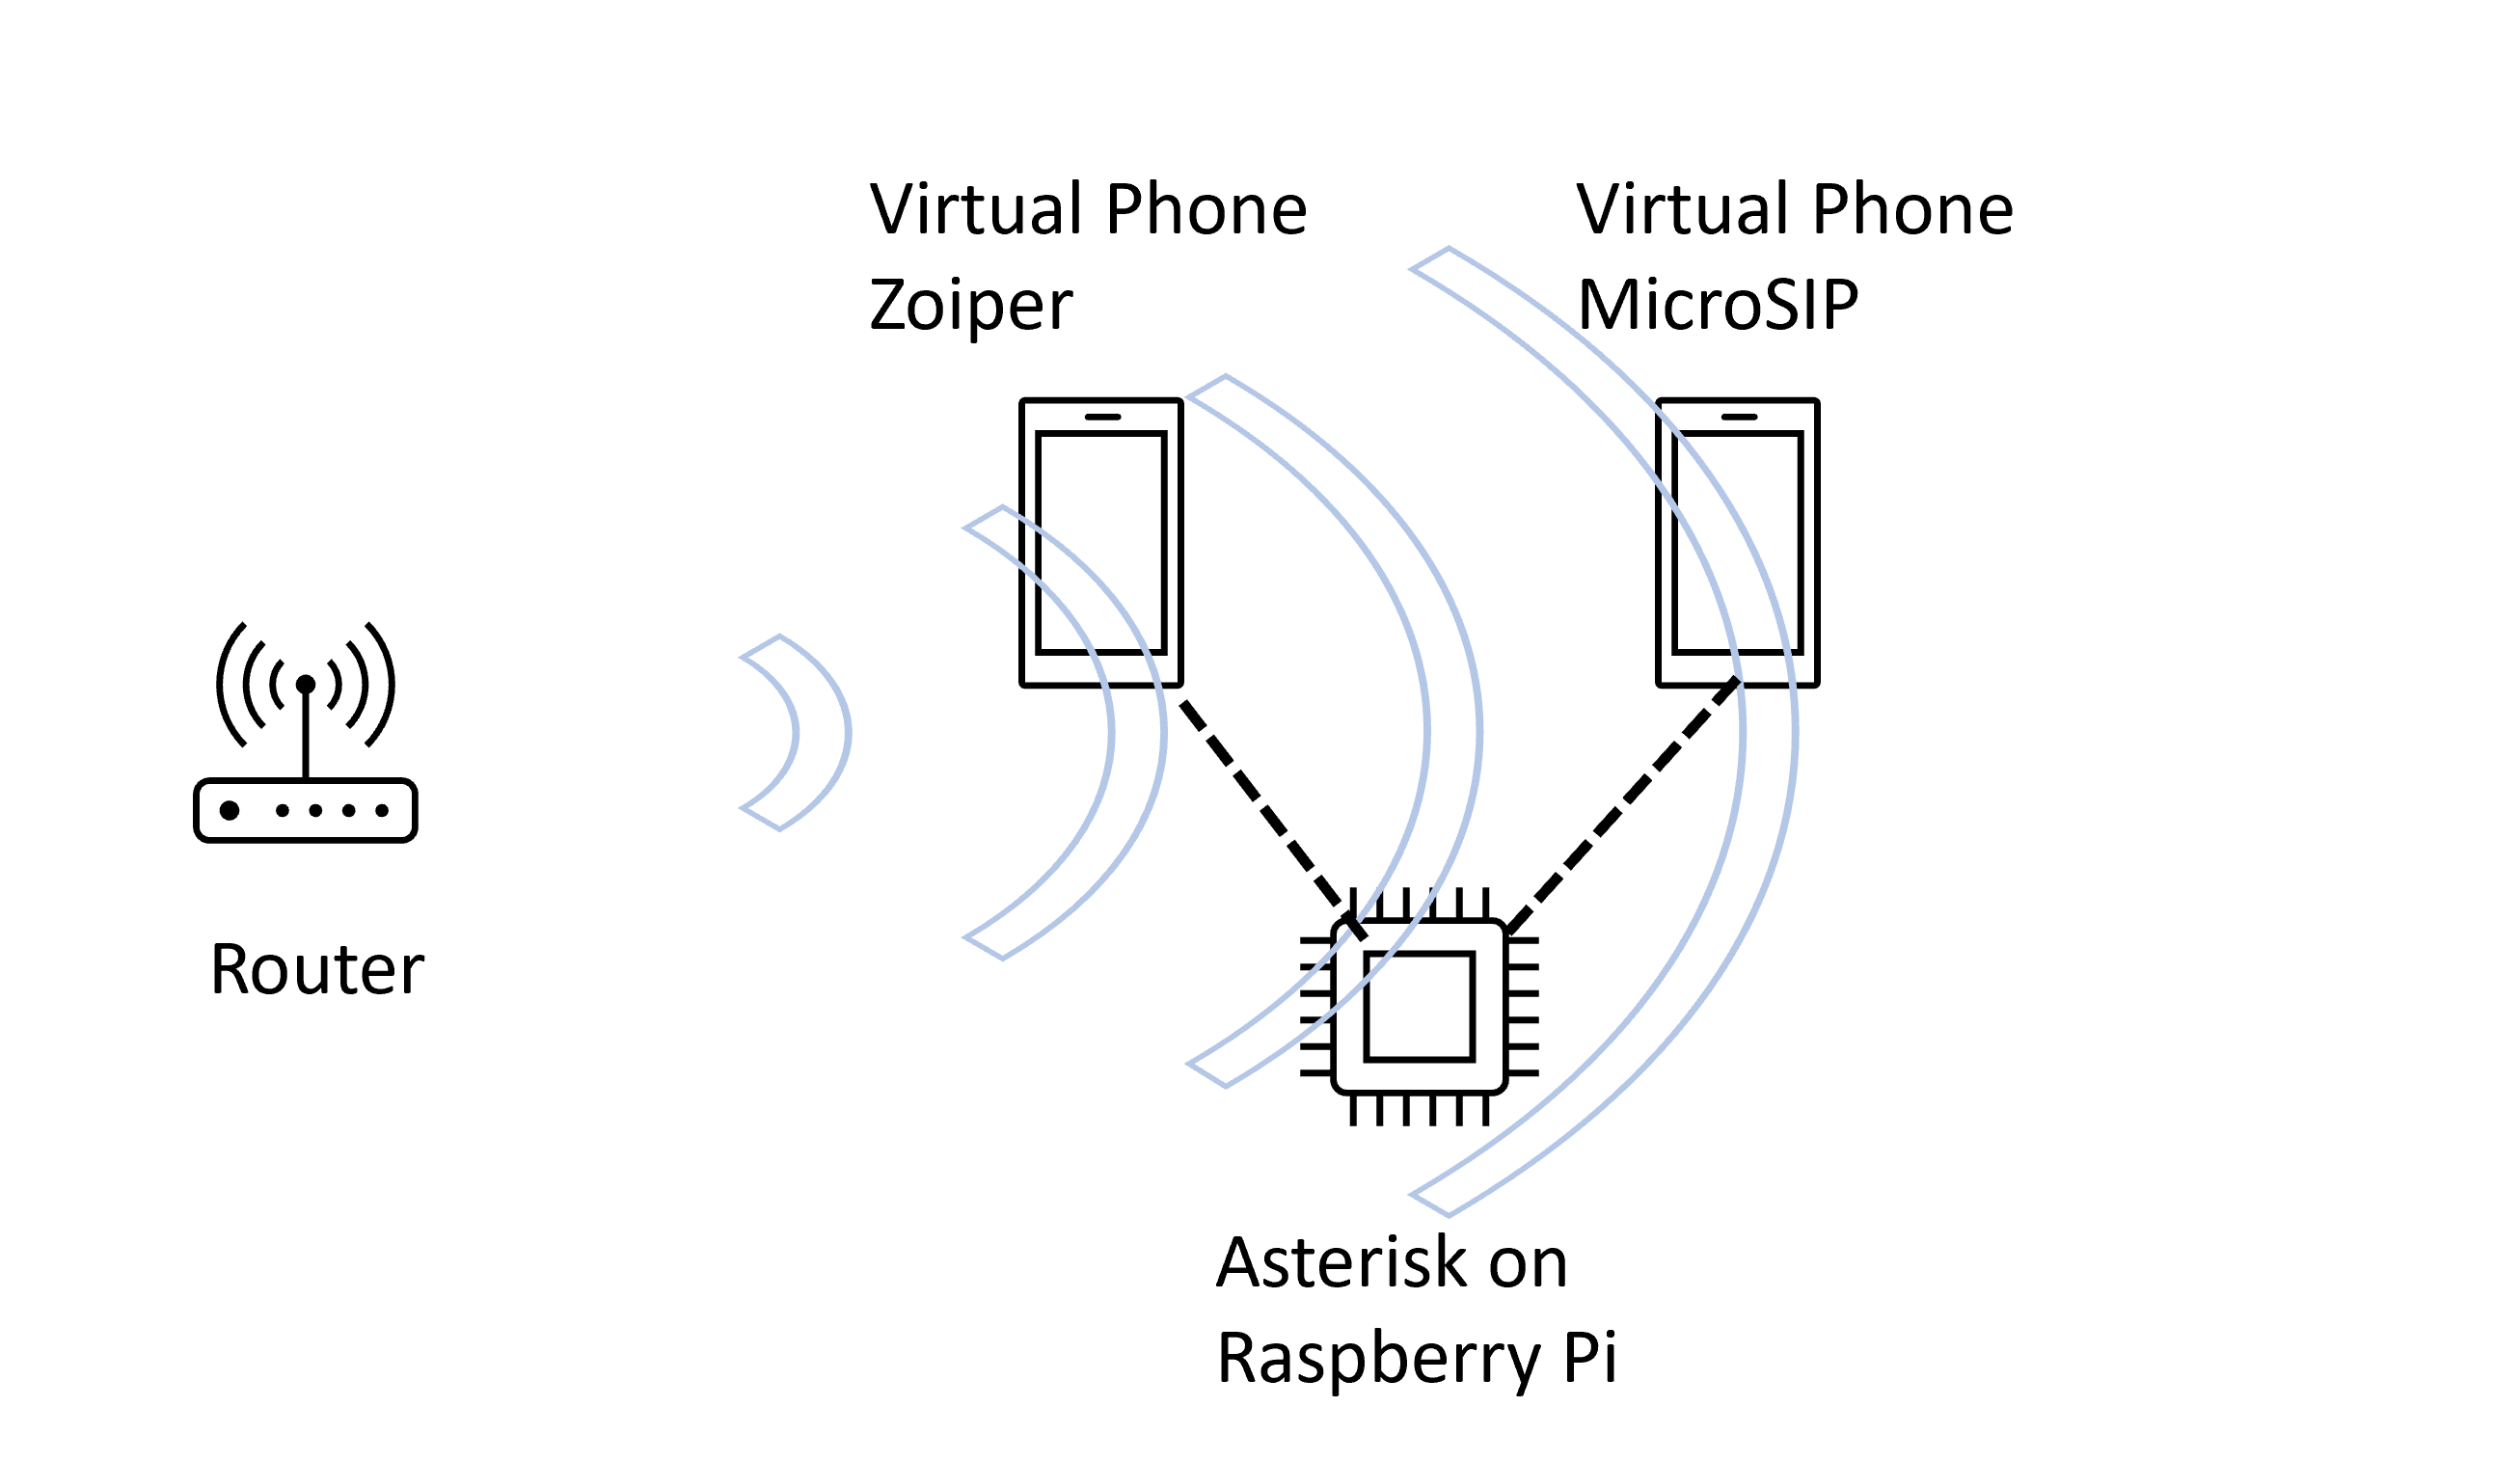
\includegraphics[width=8cm]{Images/experiment/exp1.png}}
\caption{Simplified Scenario}
\label{fig:topo}
\end{figure}

The SIP process starts with registration. All SIP terminals as User Agents should register with the registration server to inform their location, session capability, and other information.

Usually, when the SIP terminal (User Agent) is powered on or configured to perform a registration operation, a registration request message (REGISTER) is sent to the registration server, carrying all the information that needs to be registered. After receiving the registration request message, the registration server sends a response message to the terminal to inform it that the request message has been received. If the registration is successful, it will send a "200 OK" message to the terminal. However, the most common response is a "401 Unauthorized" message because authorization is required in most of the implantations for security purposes. As shown in Figure 2.


The SIP protocol adopts the Client-Server pattern, in which the calls are established between User Agents through the proxy server.


\begin{figure}[htbp]
  \centering
  \begin{minipage}[b]{0.3\textwidth}
    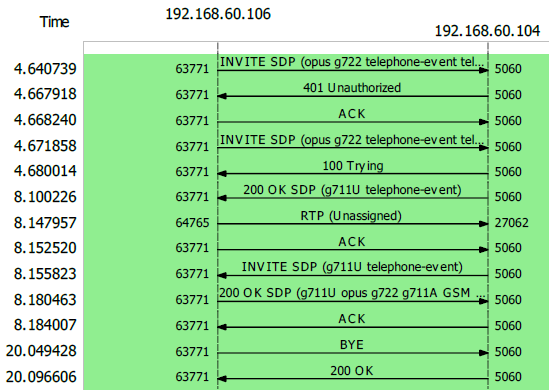
\includegraphics[width=\textwidth]{Images/experiment/a1.png}
    \caption{Zoiper to Asterisk}
  \end{minipage}
  \hfill
  \begin{minipage}[b]{0.3\textwidth}
    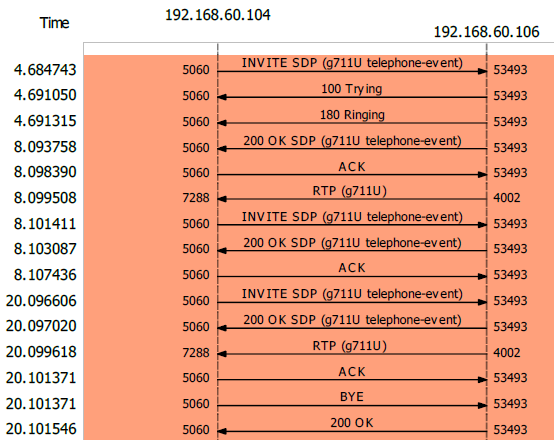
\includegraphics[width=\textwidth]{Images/experiment/a2.png}
    \caption{Zoiper to MicroSIP}
  \end{minipage}
\end{figure}


	
	
	%%
	%% The future directions  section
	\section{Future Work} \label{sec:future-work}
    While this may act as a basic foundation for proving the efficacy of the Raspberry Pi as a cheap means to implement IP-PBX software, there are several means of expanding upon this work.
    \subsection{Further Testing}
        More experiments can be performed to determine the limitations that Raspberry Pis can prove to have when running IP-PBX software. A major test would be stressing the Pi by seeing how many calls it can handle in situations where bandwidth is plentiful, with the CPU and RAM of the Pi being the major bottlenecks at that point. This same test could be performed using different models of the Pi to see how the difference in CPU and RAM can affect VoIP calls. Analyzing this data could provide a way to determine the best board to purchase based on how many calls are needed to be handled.
        
        A limitation of data for outside network calls restricts current analysis. Future studies could attempt to have separate Raspberry Pis running PBX software on different networks, while allowing VoIP calls to be made between them. Data could then be collected based on test calls between these IP-PBX instances. This would prove useful in analyzing the effectiveness of the Pi in making outside network calls.
    \subsection{Horizontal Scaling}
        A powerful characteristic of cheap computers such as a Raspberry Pi is their suitability for horizontal scaling. If an institution grows large enough that one Pi cannot handle the all of the institution's VoIP calls, there are two methods of scaling up the memory and processing power available for IP-PBX services. The first is to scale the system vertically; replace the Pi with a single, more powerful computer with more memory, and either sell the Pi or reuse it for some other purpose. The second is to scale the system horizontally; connect more Raspberry Pis with the original and have them share the workload of the VoIP calls. As Raspberry Pis are inexpensive, this allows for a cheaper alternative to buying a more powerful computer. Further works can delve into whether this is a possible technique to implement with IP-PBX software, and whether or not horizontal scaling provides many benefits for IP-PBX services.	
	
	%%
	%% The Conclusion section
	\section{Conclusion} \label{sec:conclusion}
    A single Raspberry Pi with 4GB of RAM is quite capable of running IP-PBX software without any noticeable issues. However, configuring the software to allow for VoIP calls can be quite complicated, and requires a great deal of outside instruction to fully understand. As well, a vital component of using the Raspberry Pi for these purposes is considering the network involved. If the Pi or VoIP devices are in areas with weak signal strength, jitter can grow rapidly, packet loss can begin to noticeably occur, connections can be dropped abruptly, and delays can become much more noticeable. If these effects occur, either due to weak signal strength or due to other possible issues, call quality can suffer dramatically. Consideration is required to install a usable and useful IP-PBX system for VoIP calls.
	
	%%
	%% The next two lines define the bibliography style to be used, and
	%% the bibliography file.
	\bibliographystyle{IEEEtran}
	\bibliography{ref}
	
	%%
	%% If your work has an appendix, this is the place to put it.
	\appendices
	\section{Installation of Raspberry Pi OS}	\label{sec:run-raspberry}
	To install Raspberry Pi OS on ``Raspberry Pi 4 from CanaKit'', you will need to download \textbf{`Raspberry Pi Imager'} from the website \href{https://www.raspberrypi.com/software/}{here}. The \textbf{`Raspberry Pi Imager'} is supported by all OS (Mac/Windows/Linux). 
	
	\subsection{Installation of Raspberry Pi Imager on Mac}
		\begin{itemize}[leftmargin=1.7cm]
			\item[\textbf{Step 1:}] Download Raspberry Pi Imager from \href{https://downloads.raspberrypi.org/imager/imager_latest.dmg}{here}
			\item[\textbf{Step 2:}] Open/Install ``imager\_x.x.x.dmg''
			\item[\textbf{Step 3:}] Run application "Raspberry Pi Imager"\\
				\begin{minipage}{\textwidth}
					\vspace{2mm}
					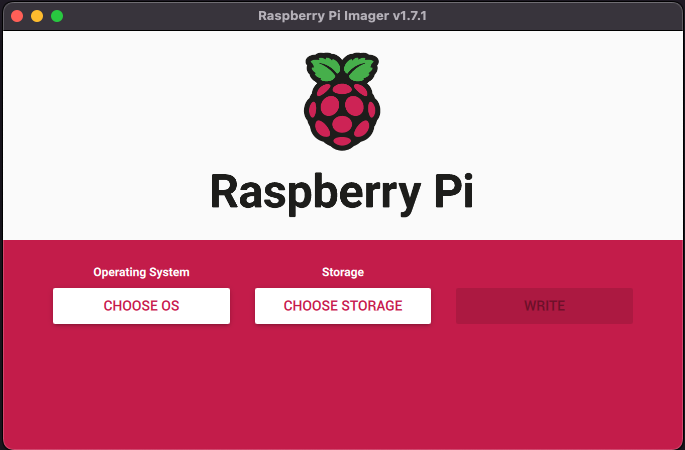
\includegraphics[scale=0.35]{Images/raspberry_pi/app.png}
					\vspace{2mm}
				\end{minipage}
			\item[\textbf{Step 4:}] Click on ``CHOOSE OS'' and Select \textbf{``Raspberry Pi OS (32-bit) Desktop''}\\
				\begin{minipage}{\textwidth}
					\vspace{2mm}
					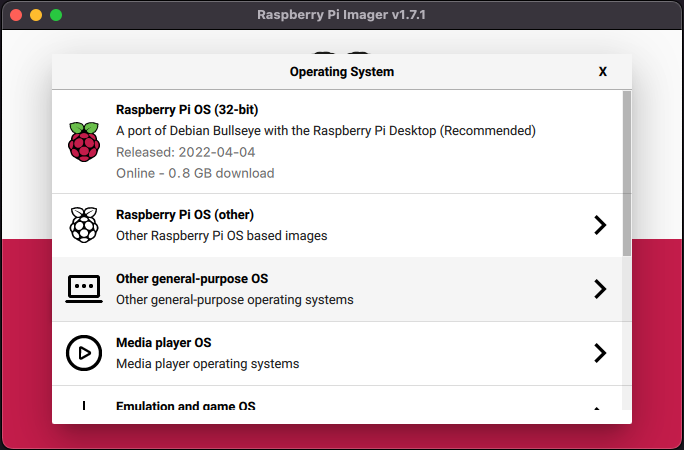
\includegraphics[scale=0.35]{Images/raspberry_pi/choose-os.png}
					\vspace{2mm}
				\end{minipage}
			\item[\textbf{Step 5:}] Click on ``CHOOSE STORAGE'' (\textbf{NOTE:} Please make sure you select correct SD card with is in Raspberry Pi 4)
			\item[\textbf{Step 6:}] Click on ``WRITE''
			\item[\textbf{Step 7:}] Wait untill writting is complete.
		\end{itemize}
	
	\subsection{Login to Raspberry Pi OS}
		At the begining  the user name of the OS is \textbf{``pi''} and password is \textbf{``raspberry''}. (\textbf{NOTE:} For this project we did \textbf{NOT} change any default user and password.)
	
	\subsubsection{Accessing Raspberry Pi}	\label{subsubsec:ssh}
		There are multiple ways you can access the \textbf{``pi''} user.  
		\begin{itemize}[leftmargin=1.2cm]
			\item Accessing through SSH \\
				To access \textbf{``pi''} user using SSH connection you need to make sure that your computer and Raspberry Pi are in same Internet connection. In this project it is ``eduroam'' connection. To setup ``eduroam'' connection into your newly install Raspberry Pi OS, please follow the instruction from \hyperref[sec:run-eduroam]{Section \ref{sec:run-eduroam}}.
				\begin{itemize}[leftmargin=1.3cm]
					\item[\textbf{Step 1:}] Open Terminal in your local computer \\
						\begin{minipage}{\textwidth}
							\vspace{2mm}
							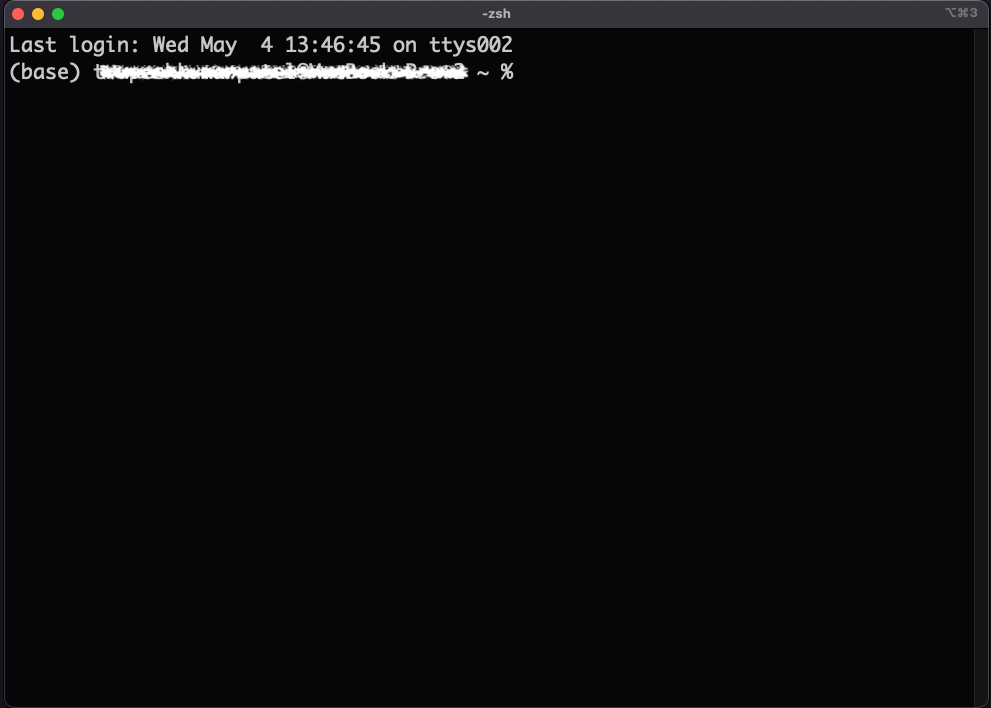
\includegraphics[scale=0.35]{Images/raspberry_pi/ssh_login/open_iterm.png}
							\vspace{2mm}
						\end{minipage}
					\item[\textbf{Step 2:}] Type command ``ssh pi@10.127.227.112'' <-- here `10.127.227.112' is IP address of Raspberry Pi, in your case might be different.\\
						\begin{minipage}{\textwidth}
							\vspace{2mm}
							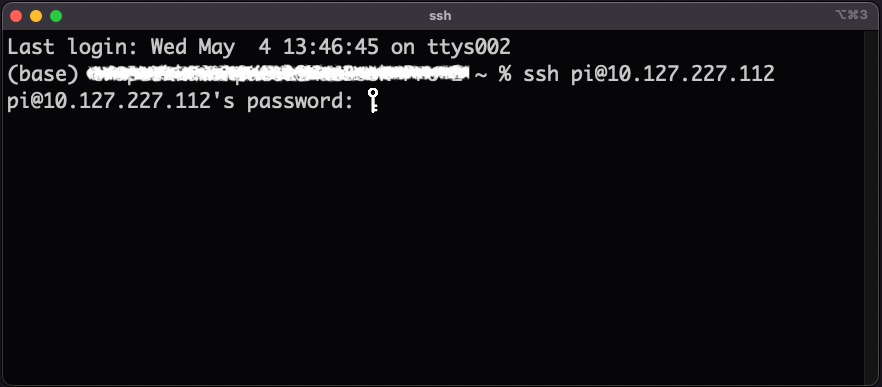
\includegraphics[scale=0.35]{Images/raspberry_pi/ssh_login/login.png}
							\vspace{2mm}
						\end{minipage}
					\item[\textbf{Step 3:}] Enter the password ``raspberry''. Please enter the password that you set if you have, else it is going to be same as the authors.\\
						\begin{minipage}{\textwidth}
							\vspace{2mm}
							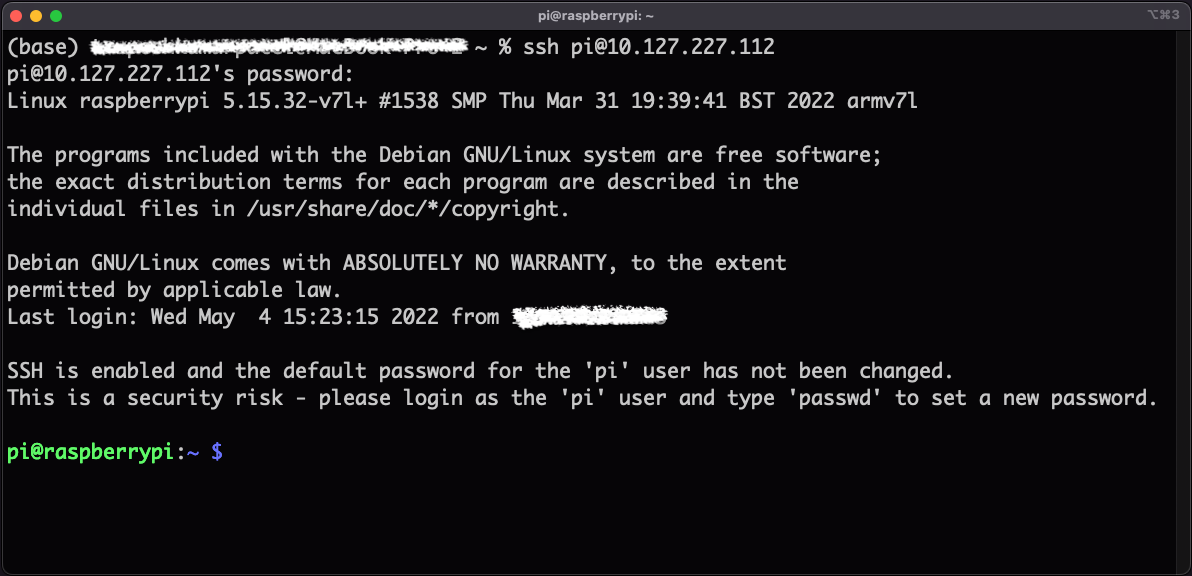
\includegraphics[scale=0.35]{Images/raspberry_pi/ssh_login/after_login.png}
							\vspace{2mm}
						\end{minipage}
				\end{itemize}
		\end{itemize}
	\section{Connect to eduroam}	\label{sec:run-eduroam}
	 To re-run the project, you have to connect your Raspberry Pi with ``eduroam'' network at The Univeristy of Alabama. Now, if you have freshly install the Raspberry Pi OS, then you need to run the script called \textbf{``config\_eduroam.sh''}, which can be found \href{https://github.com/TrupeshKumarPatel/IoT_RaspberryPi/tree/main/source_code/eduroam_config}{here}. 
	 
\subsection{Configure Raspberry Pi for eduroam}
		\begin{itemize}[leftmargin=1.8cm]
			\item[\textbf{Step 1:}] Login to the Raspberry Pi as user ``pi'' %(\textbf{Note:} You can follow steps from \hyperref[subsubsec:ssh]{Section \ref{subsubsec:ssh}}.)
			\item[\textbf{Step 2:}] Type command ``{\fontfamily{cmtt}\selectfont{git clone https://github\\.com/TrupeshKumarPatel/IoT\_RaspberryPi.\\git}}''\\
				\begin{minipage}{\textwidth}
					\vspace{2mm}
					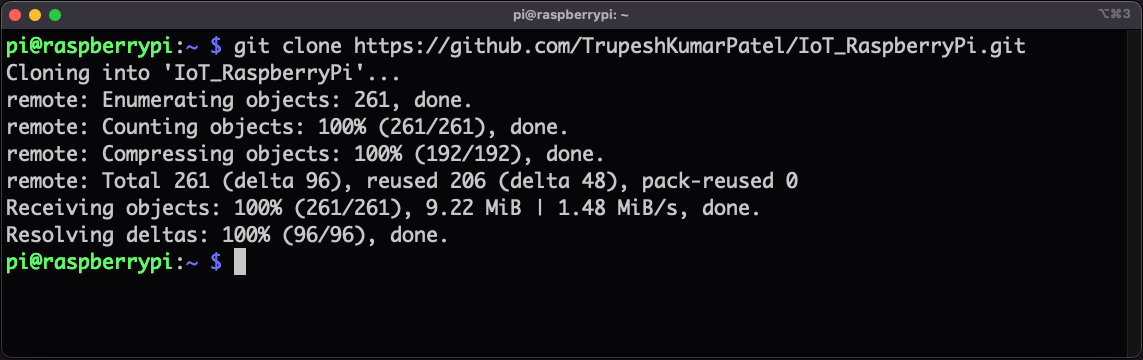
\includegraphics[scale=0.17]{Images/raspberry_pi/eduroam_config/clone_git.png}
					\vspace{2mm}
				\end{minipage}
			\item[\textbf{Step 3:}] Type command ``{\fontfamily{cmtt}\selectfont{sudo su}}'' ~\danger\textbf{NOTE} ~This com\\mand to get sudo access to Raspberry Pi \danger\\
				\begin{minipage}{\textwidth}
					\vspace{2mm}
					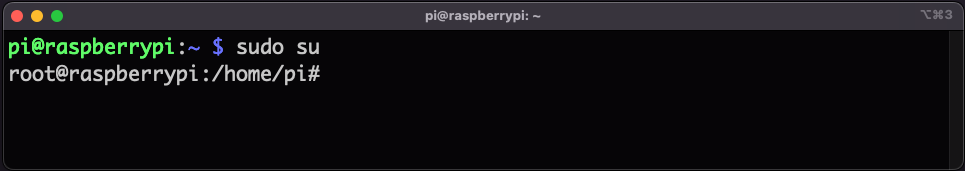
\includegraphics[scale=0.2]{Images/raspberry_pi/eduroam_config/sudo_login.png}
					\vspace{2mm}
				\end{minipage}
			\item[\textbf{Step 4:}] Type command ``{\fontfamily{cmtt}\selectfont{chmod +x IoT\_Raspberry\\Pi/source\_code/eduroam\_config/config\\\_eduroam.sh}}''\\
				\begin{minipage}{\textwidth}
					\vspace{2mm}
					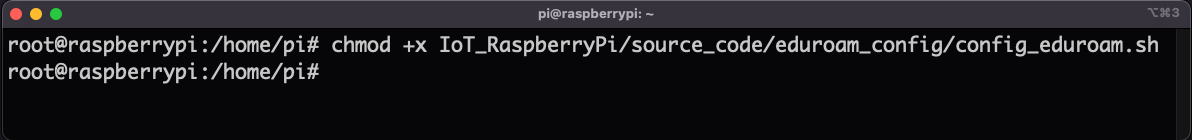
\includegraphics[scale=0.16]{Images/raspberry_pi/eduroam_config/permission_x.png}
					\vspace{2mm}
				\end{minipage}
			\item[\textbf{Step 5:}] Type command ``{\fontfamily{cmtt}\selectfont{./IoT\_RaspberryPi/sourc\\e\_code/eduroam\_c\\onfig/config\_eduroam.sh}}''
			\item[\textbf{Step 6:}] Enter your crimson email address
			\item[\textbf{Step 7:}] Enter your crimson password\\
				\begin{minipage}{\textwidth}
					\vspace{2mm}
					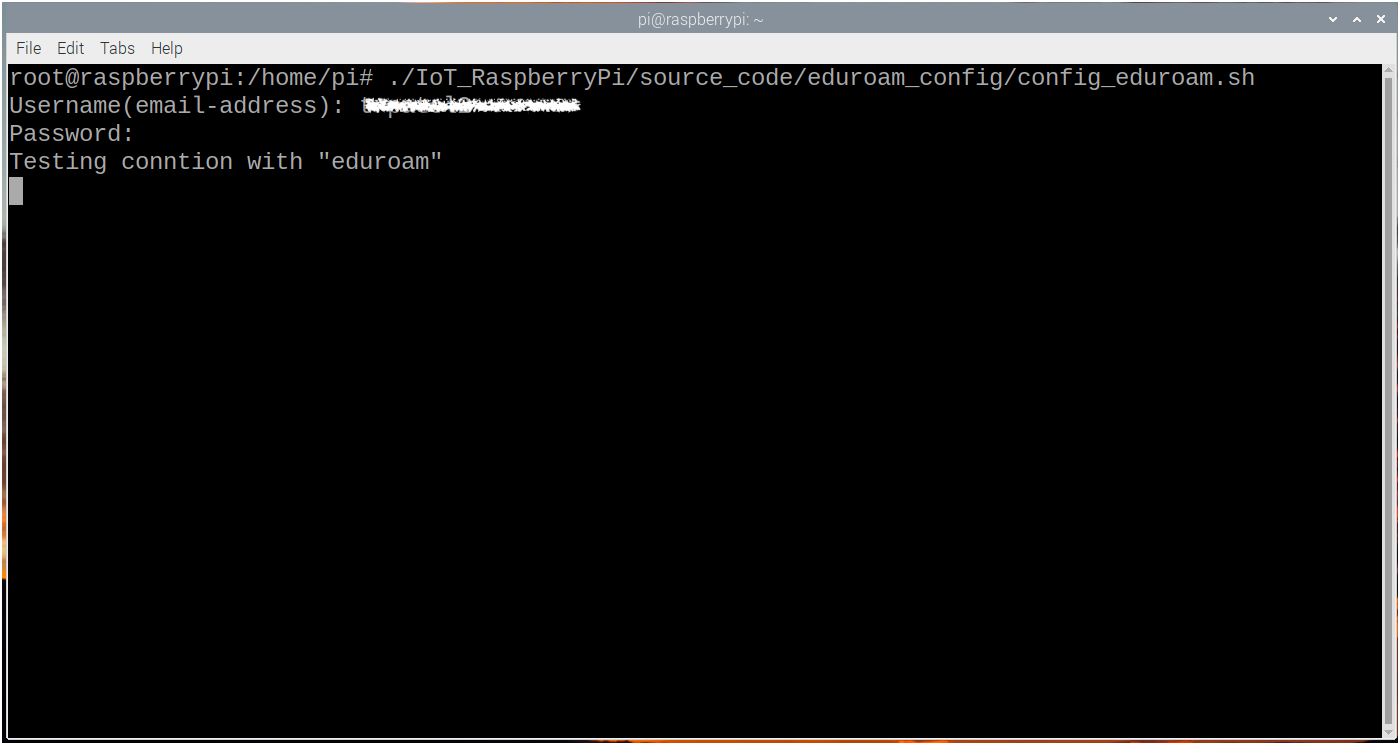
\includegraphics[scale=0.14]{Images/raspberry_pi/eduroam_config/run_eduroam_conf.png}
					\vspace{2mm}
				\end{minipage}
			\item[\textbf{Step 8:}] Now wait for your Raspberry Pi to restart
		\end{itemize}
	\section{Installation of Asterisk}	\label{sec:run-asterisk}
	To install Asterisk same as this project authors, please follow below instructions: (\textbf{Note:} Here author installing Asterisk from source code. You can also follow the installation video from \href{https://www.youtube.com/watch?v=52sEPVPV9JE&list=PLruX0IBTg1G4Auvo5YhoJKgskmMP7b8bJ&index=4&ab_channel=InnovateAsterisk}{InnovationAsterisk})
	
	\subsection{Asterisk Installation from the Source Code}
		\begin{itemize}[leftmargin=1.7cm]
			\item[\textbf{Step 1:}] Type command ``{\fontfamily{cmtt}\selectfont{wget http://downloads.asterisk.org/pub/telephony/asterisk/asterisk-18-curren\\t.tar.gz}}''\\
				\begin{minipage}{\textwidth}
					\vspace{2mm}
					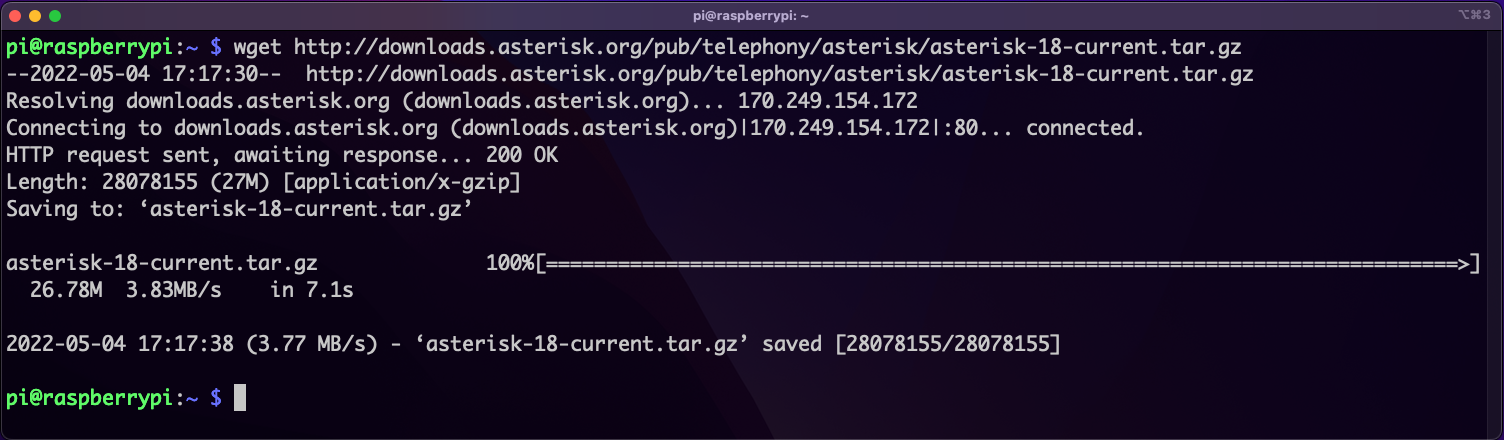
\includegraphics[scale=0.3]{Images/raspberry_pi/asterisk_install/wget.png}
					\vspace{2mm}
				\end{minipage}
			
			\item[\textbf{Step 2:}] Type command ``{\fontfamily{cmtt}\selectfont{sudo apt-get update}}''
			\item[\textbf{Step 3:}] Type command ``{\fontfamily{cmtt}\selectfont{sudo apt-get upgrade}}''
			\item[\textbf{Step 4:}] Type command ``{\fontfamily{cmtt}\selectfont{sudo apt-get install ntp}}''
			\item[\textbf{Step 5:}] Type command ``{\fontfamily{cmtt}\selectfont{sudo apt-get install speex speex* libspeex-dev libspeexdsp-dev}}''
			\item[\textbf{Step 6:}] Type command ``{\fontfamily{cmtt}\selectfont{sudo apt-get install libspeex-dev libspeexdsp-dev speex speex-doc}}''
			\item[\textbf{Step 7:}] Type command ``{\fontfamily{cmtt}\selectfont{sudo apt-get install xmlstarlet libopus-dev libopusfile-dev}}'' <-- (\textbf{NOTE:} This optional if you don't want browser-base telephony, here author did not do this)
			
			\item[\textbf{Step 8:}] Type command ``{\fontfamily{cmtt}\selectfont{tar -xvf asterisk-18-current.tar.gz}}'' <-- This command will extract all the source file into folder called ``asterisk-18.x.x'' (\textbf{Note:} here `x' could be any number based of current relese/download)
			
			\item[\textbf{Step 9:}] Type command ``{\fontfamily{cmtt}\selectfont{cd asterisk-18.x.x}}'' <-- (\textbf{Note:} here `x' could be any number based of current relese/download)
			
			\item[\textbf{Step 10:}] Type command ``{\fontfamily{cmtt}\selectfont{sudo contrib/scripts/install\_prereq install}}'' <-- This will check all the prerequisites of Asterisk. This command will ask few promps to set configurations
					\begin{enumerate}
						\item Telephone code : Type ``{\fontfamily{cmtt}\selectfont{1}}'' for US
					\end{enumerate}
			\item[\textbf{Step 11:}] Type command ``{\fontfamily{cmtt}\selectfont{sudo ./configure --libdir=/usr/lib --with-pjproject-bundled}}''
			
			\item[\textbf{Step 12:}] Type command ``{\fontfamily{cmtt}\selectfont{sudo make menuselect}}'' <-- Please watch this \href{https://www.youtube.com/watch?v=52sEPVPV9JE&list=PLruX0IBTg1G4Auvo5YhoJKgskmMP7b8bJ&index=4&ab_channel=InnovateAsterisk}{video}) from InnovateAsterisk for more details.

			\item[\textbf{Step 13:}] Type command ``{\fontfamily{cmtt}\selectfont{sudo make}}''
			\item[\textbf{Step 14:}] Type command ``{\fontfamily{cmtt}\selectfont{sudo make install}}''
			\item[\textbf{Step 15:}] Type command ``{\fontfamily{cmtt}\selectfont{sudo make samples}}'' <-- This will create all default Asterisk configuration files\\\\
			\danger\textbf{NOTE:} \textbf{Step 16-17} is only required if you haven't downloaded ``IoT\_RaspberryPi'' GitHub repository from \href{https://github.com/TrupeshKumarPatel/IoT_RaspberryPi}{here}  \danger\\
			\item[\textbf{Step 16\danger:}] Type command ``{\fontfamily{cmtt}\selectfont{cd ~}}''
			\item[\textbf{Step 17\danger:}] Type command ``{\fontfamily{cmtt}\selectfont{git clone https://github.com/TrupeshKumarPatel/IoT\_RaspberryPi.git}}''\\
				\begin{minipage}{\textwidth}
					\vspace{2mm}
					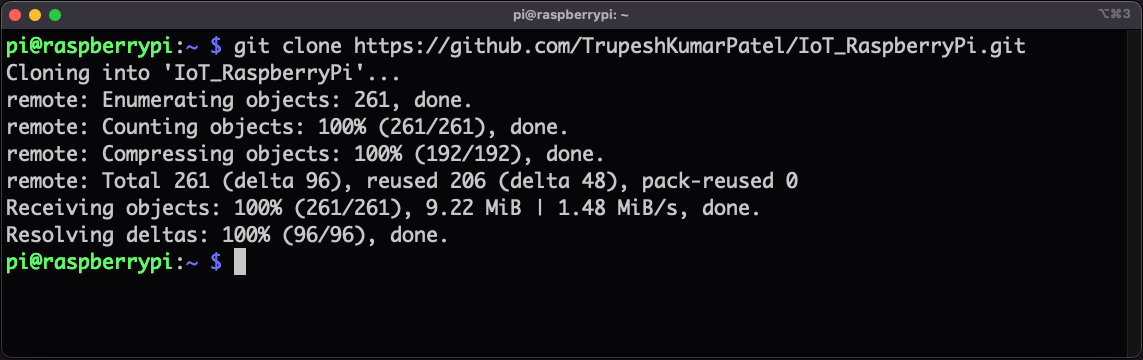
\includegraphics[scale=0.35]{Images/raspberry_pi/eduroam_config/clone_git.png}
					\vspace{2mm}
				\end{minipage}
			\item[\textbf{Step 18:}] Types command ``{\fontfamily{cmtt}\selectfont{sudo cp -R ~/IoT\_RaspberryPi/source\_code/asterisk\_config/* /etc/asterisk/}}''
		\end{itemize}

\pagebreak
\section{Command of Asterisk}	\label{sec:command-asterisk}
	Now, after following instruction from \hyperref[sec:run-asterisk]{Section \ref{sec:run-asterisk}}, you should be able to run asterisk commands.
	\begin{itemize}
		\item To check the status of Asterisk\\
		Type command ``{\fontfamily{cmtt}\selectfont{sudo service asterisk status}}''
		\item To start the Asterisk\\
		Type command ``{\fontfamily{cmtt}\selectfont{sudo service asterisk start}}''
		\item To restart the Asterisk\\
		Type command ``{\fontfamily{cmtt}\selectfont{sudo service asterisk restart}}''
		\item To stop the Asterisk\\
		Type command ``{\fontfamily{cmtt}\selectfont{sudo service asterisk stop}}''
		\item To access CLI of the Asterisk\\
		Type command ``{\fontfamily{cmtt}\selectfont{sudo asterisk -r}}''\\
			\begin{minipage}{\textwidth}
				\vspace{2mm}
				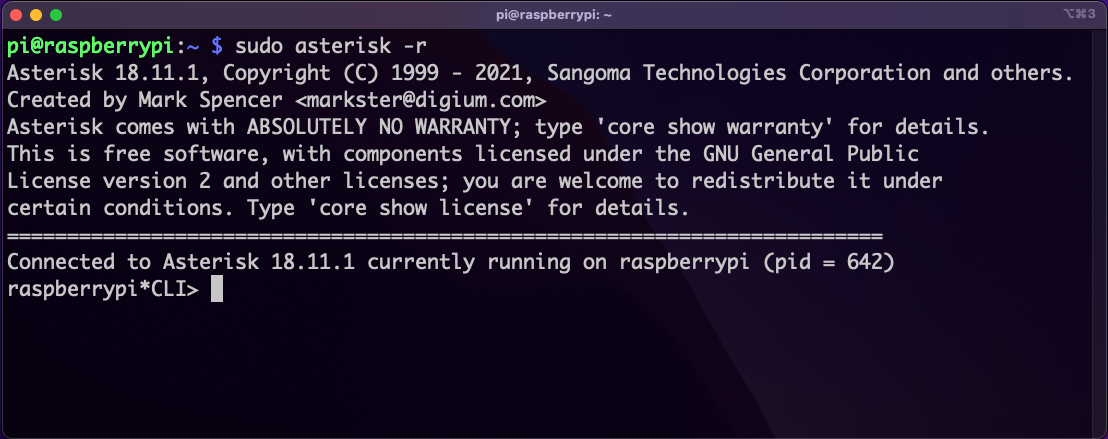
\includegraphics[scale=0.35]{Images/raspberry_pi/asterisk_install/CLI.png}
				\vspace{2mm}
			\end{minipage}
		\item To see all peers\\
		Type command ``{\fontfamily{cmtt}\selectfont{sip show peers}}''\\
			\begin{minipage}{\textwidth}
				\vspace{2mm}
				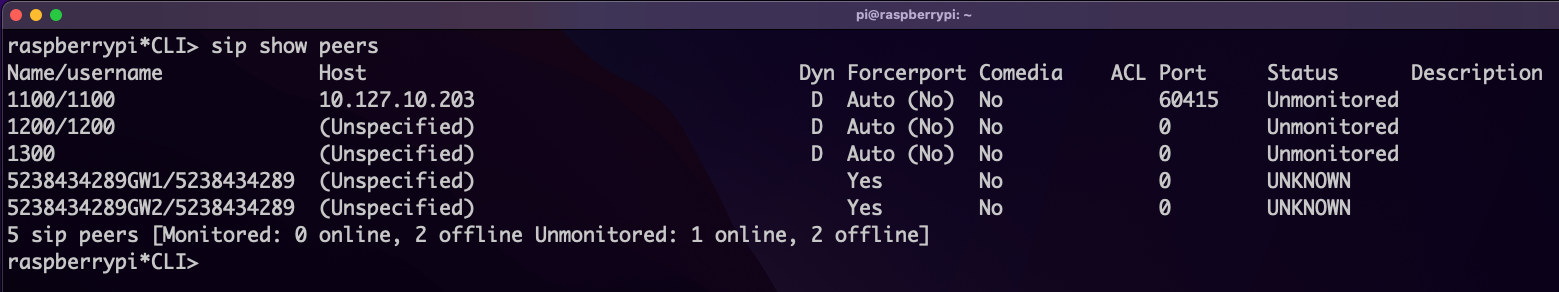
\includegraphics[scale=0.3]{Images/raspberry_pi/asterisk_install/show_peers.png}
				\vspace{2mm}
			\end{minipage}
		\item To see all users\\
		Type command ``{\fontfamily{cmtt}\selectfont{sip show users}}''\\
		\begin{minipage}{\textwidth}
			\vspace{2mm}
			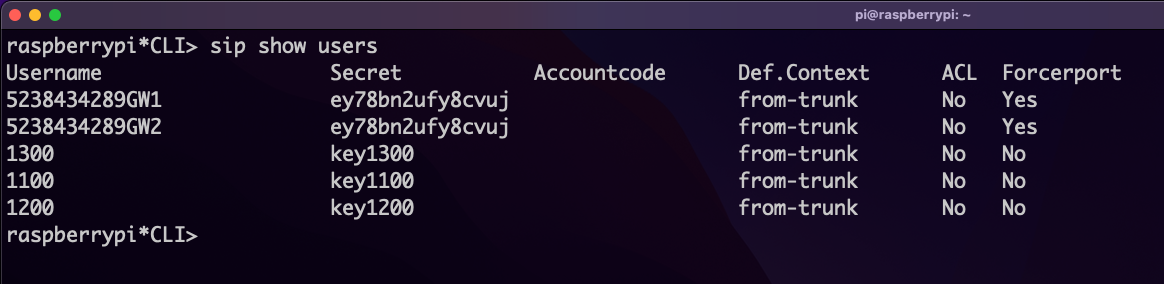
\includegraphics[scale=0.3]{Images/raspberry_pi/asterisk_install/show_users.png}
			\vspace{2mm}
		\end{minipage}
	\end{itemize}
	
	There are many Asterisk commands are available in their document offical website \href{https://wiki.asterisk.org/wiki/display/AST/Asterisk+18+Documentation}{here} and external soure \href{https://www.voip-info.org/asterisk-cli/}{here}, use it as you need.

	
\end{document}